\chapter{Implementa��o}

\section{Prot�tipo de Telas}

% Apresentar o prot�tipo do sistema, que consiste na interface preliminar contendo um conjunto de funcionalidades e telas. O prot�tipo � um recurso que deve ser adotado como estrat�gia para levantamento, detalhamento, valida��o de requisitos e modelagem de interface com o usu�rio (usabilidade).

% As telas do sistema podem ser criadas na pr�pria linguagem de desenvolvimento ou em qualquer outra ferramenta de desenho. Cada tela deve possuir uma descri��o do seu funcionamento, constando pelo menos o objetivo da tela e din�mica de navega��o (de onde � chamada e que outras telas pode chamar). A descri��o das telas deve registrar informa��es que possam ser consultadas para facilitar a implementa��o e a execu��o de testes, assim como a que requisitos funcionais se referem.

\subsection{Unity}

\subsubsection{Menu}

\begin{figure}[ht!]
	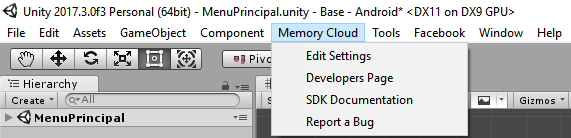
\includegraphics[width=\textwidth]{./6/menu.png}
\end{figure}

\subsubsection{Settings}

\begin{figure}[ht!]
	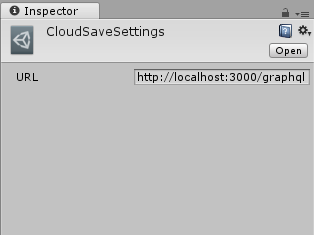
\includegraphics[width=\textwidth]{./6/settings.png}
\end{figure}

\subsection{Dashboard}

\subsubsection{Login}

\begin{figure}[ht!]
	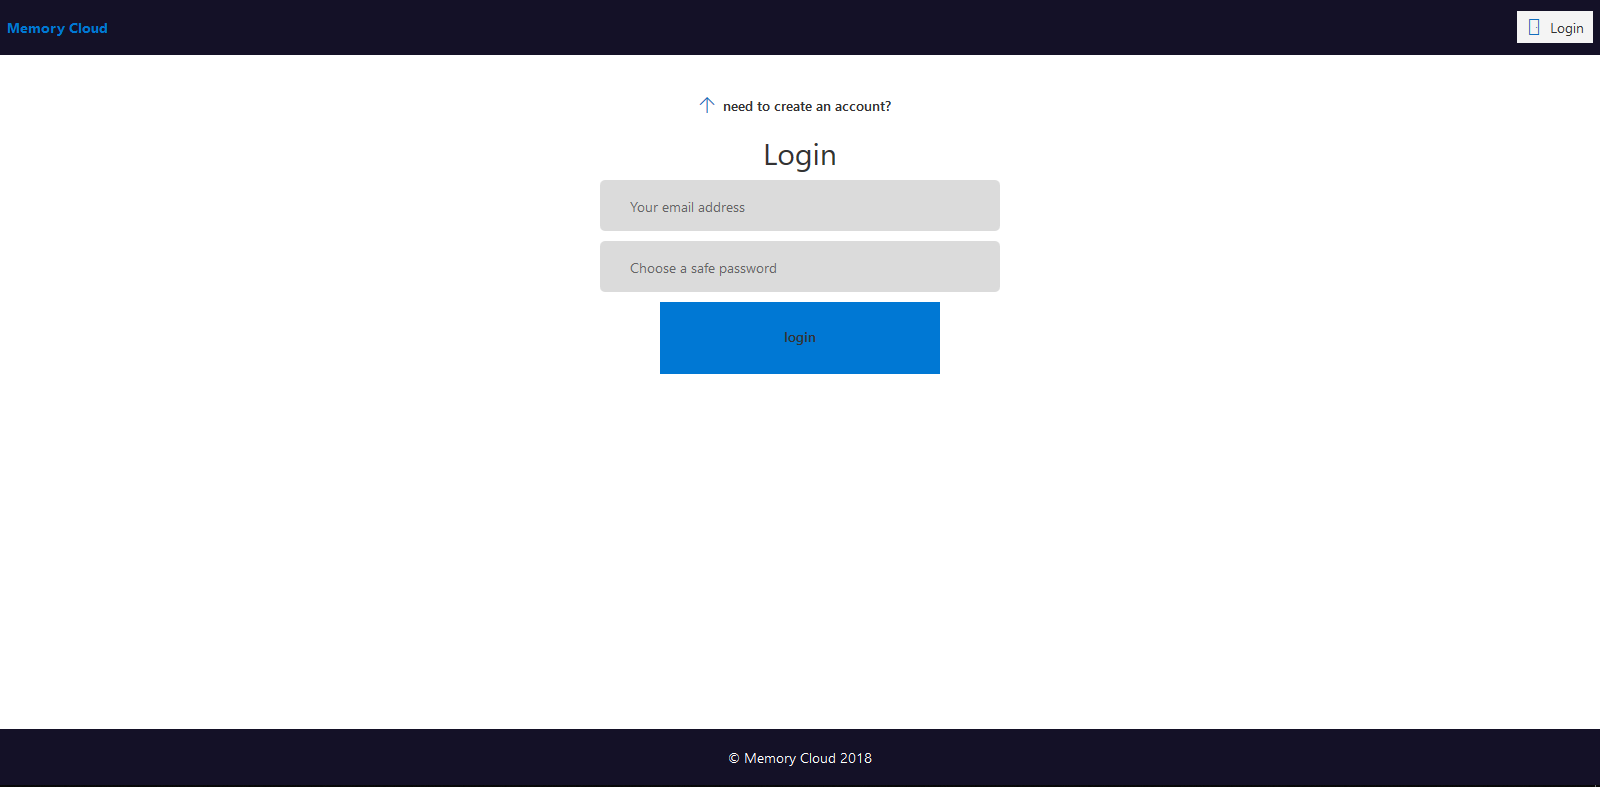
\includegraphics[width=\textwidth]{./6/login.png}
\end{figure}

\subsubsection{SignUp}

\begin{figure}[ht!]
	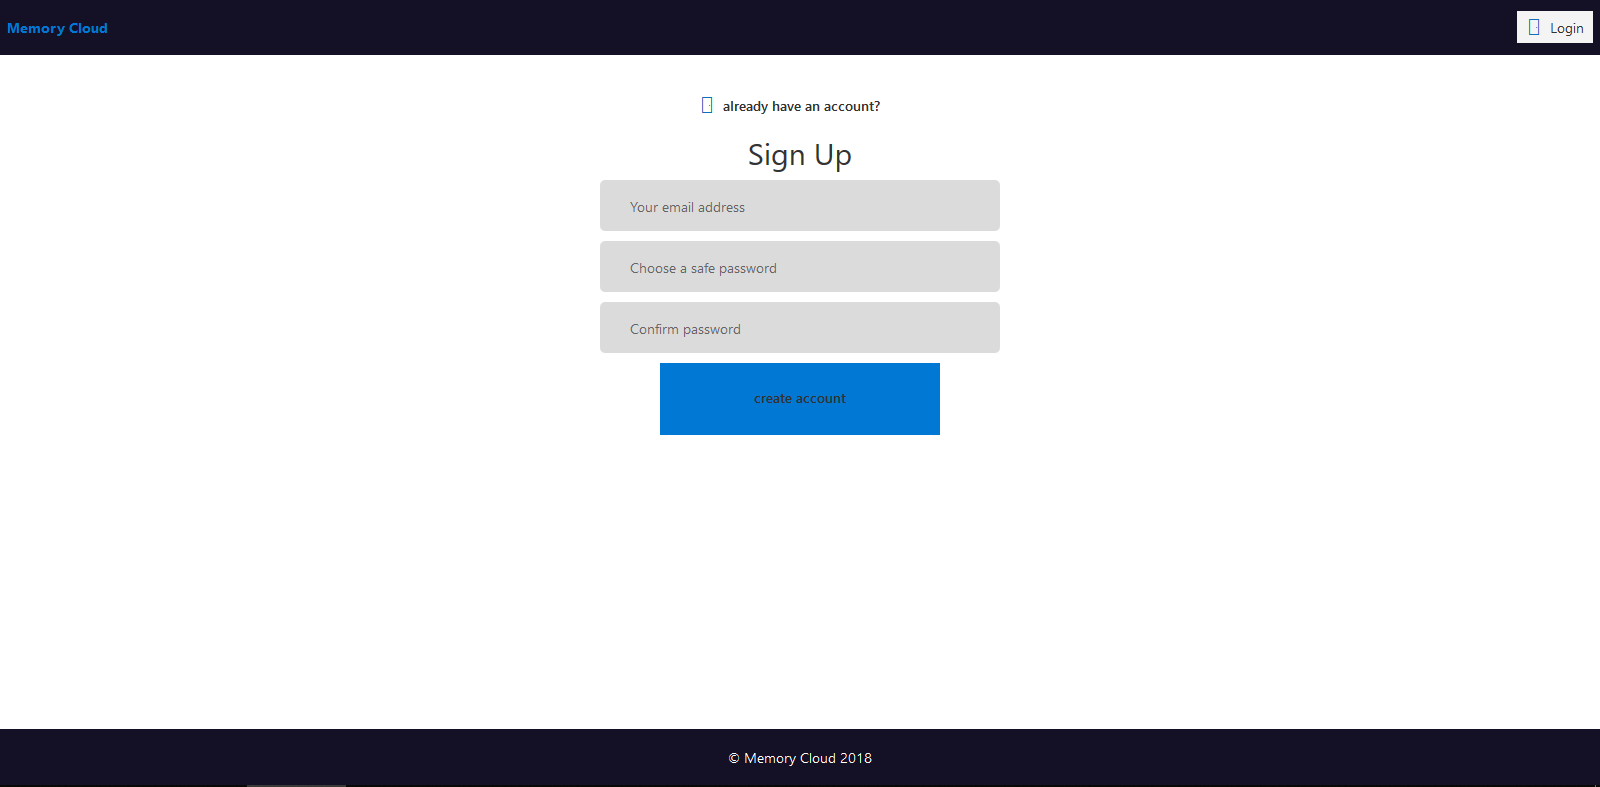
\includegraphics[width=\textwidth]{./6/signup.png}
\end{figure}

\pagebreak

\subsubsection{Games}

\begin{figure}[ht!]
	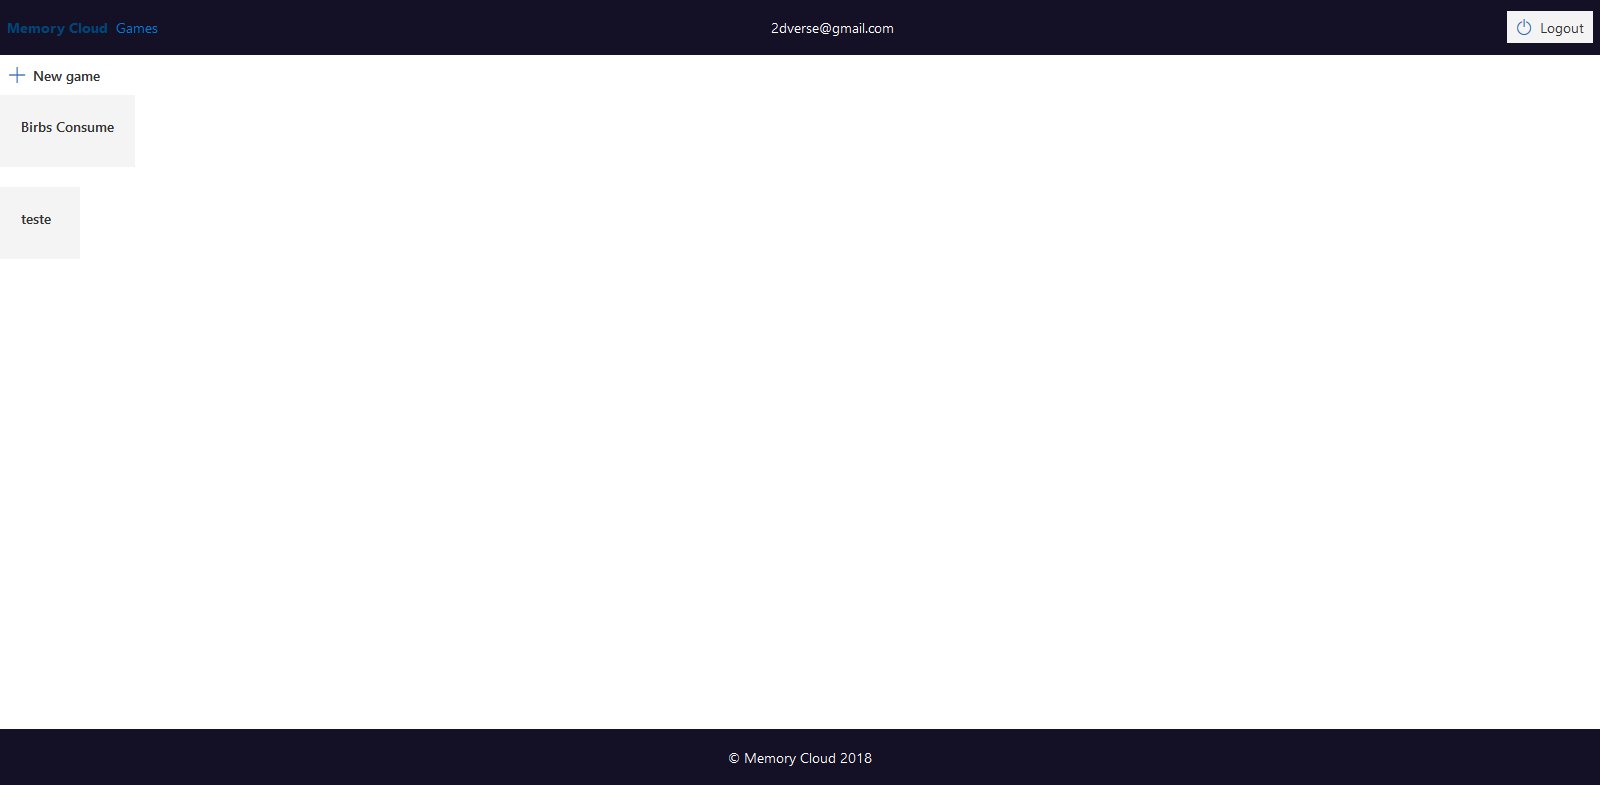
\includegraphics[width=\textwidth]{./6/games.png}
\end{figure}

\subsubsection{Game}

\begin{figure}[ht!]
	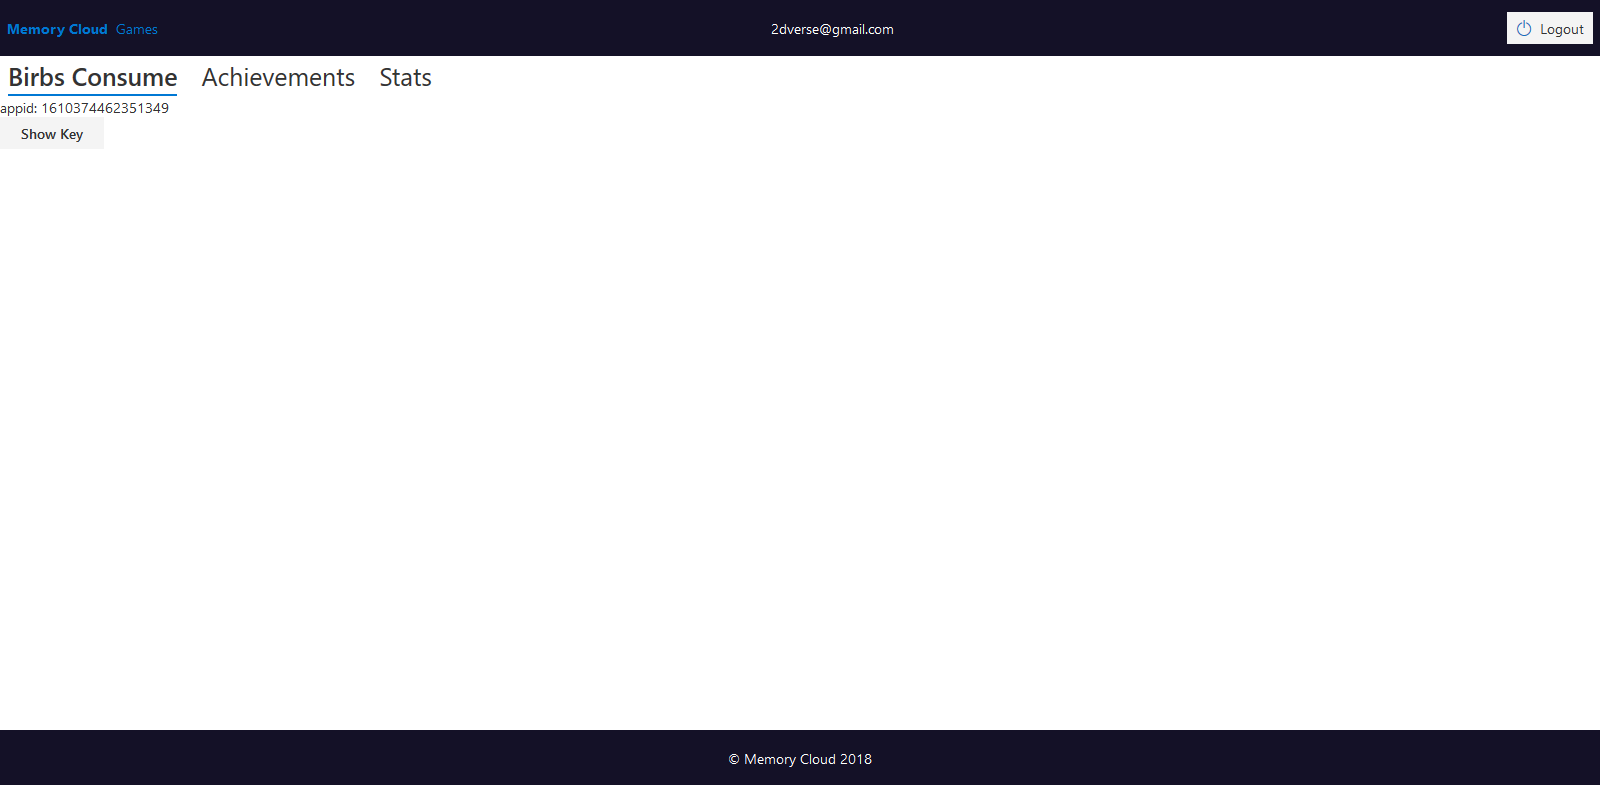
\includegraphics[width=\textwidth]{./6/game.png}
\end{figure}

\pagebreak

\subsubsection{Achievements}

\begin{figure}[ht!]
	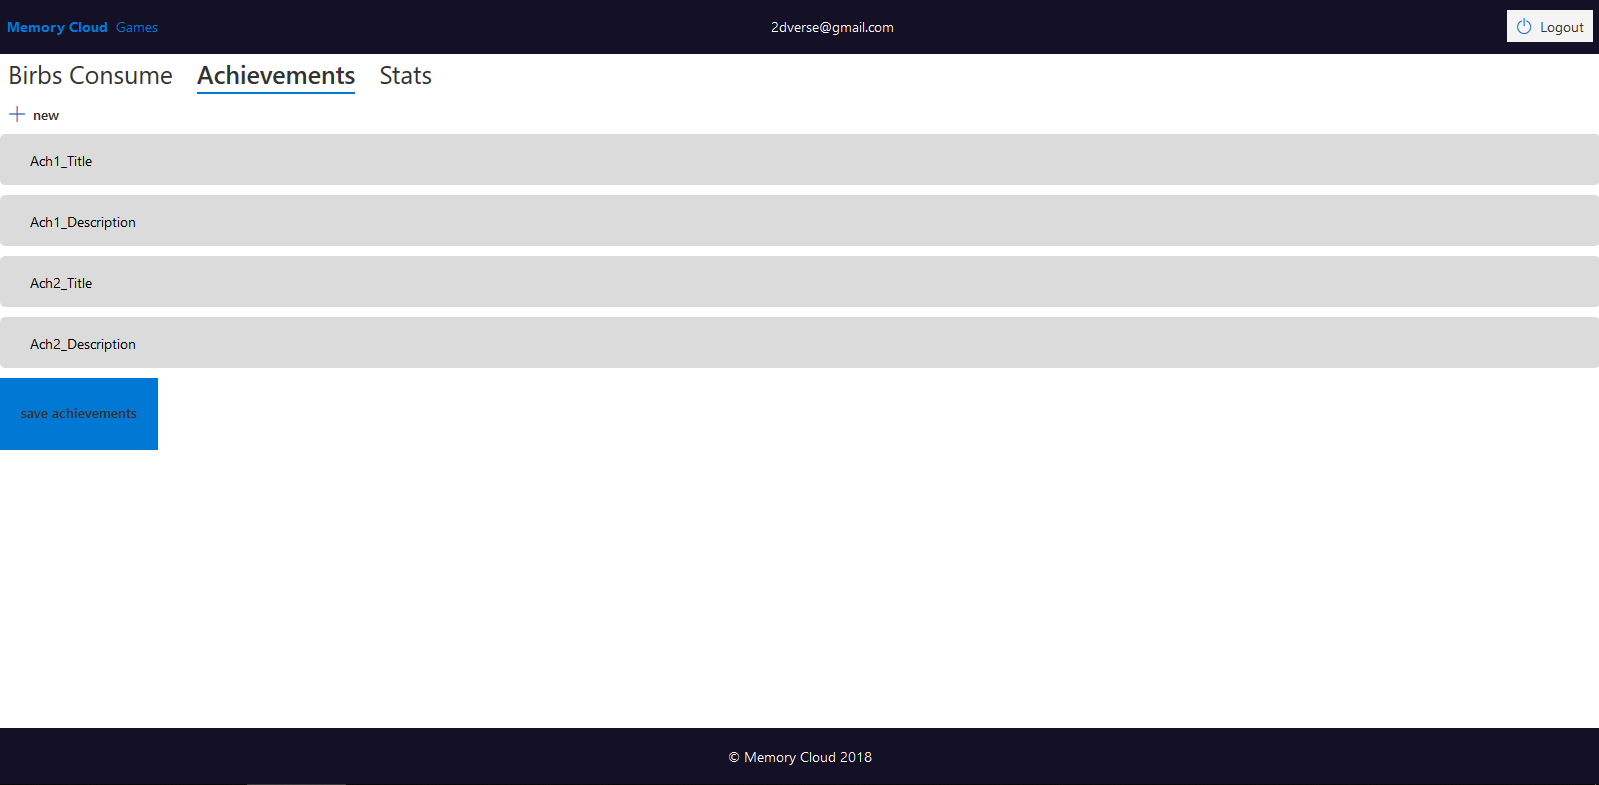
\includegraphics[width=\textwidth]{./6/achievements.png}
\end{figure}

\pagebreak

\section{Descri��o do C�digo}

\begin{figure}[ht!]
	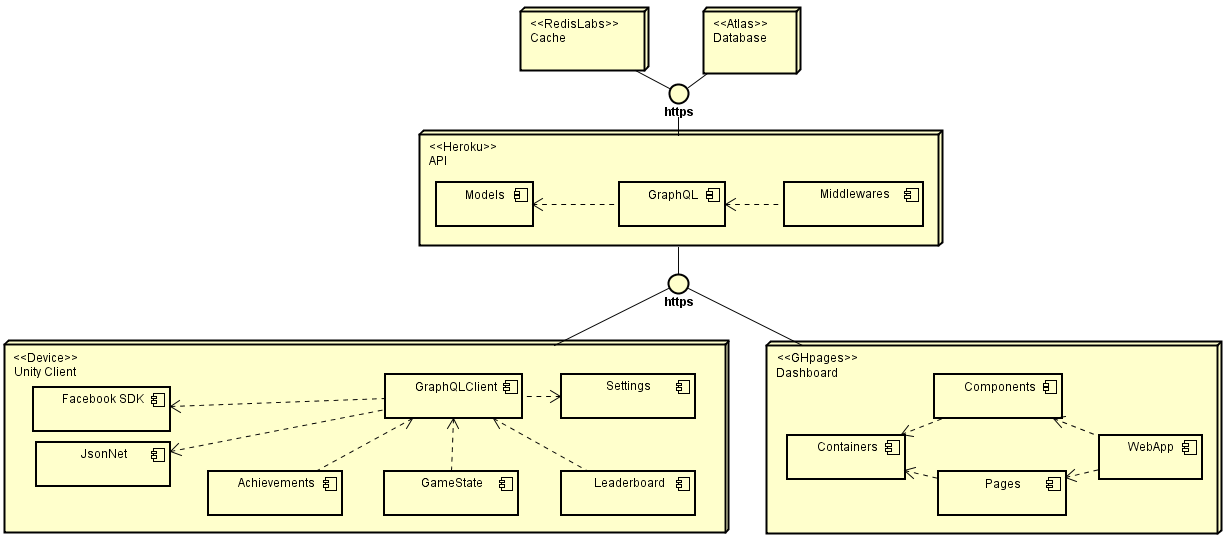
\includegraphics[width=\textwidth]{./6/diagrama.png}
\end{figure}

% Descrever o sistema quanto ao c�digo gerado. Explicar a organiza��o dos arquivos, pacotes, classes ou quaisquer estruturas utilizadas no desenvolvimento do projeto, listando os componentes criados e sua estrutura. Use diagramas (Diagrama de Componentes, Diagrama de Pacotes) para ilustrar a implementa��o. 

% Descrever tamb�m conven��es e padroniza��es para coment�rios no c�digo, nomenclatura de classes, objetos, fun��es, etc. Se necess�rio, use exemplos.
